\section{Overall description}
\subsection{Product perspective}
	\subsubsection{System interfaces}
	\label{sec:systemInterfaces}
		The system we are to develop will have some external interfaces (represented in Figure \ref{fig:systemInterfaces}) to accomplish the goals stated in section 1.3.1\todo{reference?}.
		\begin{figure}[h]
			\centering
			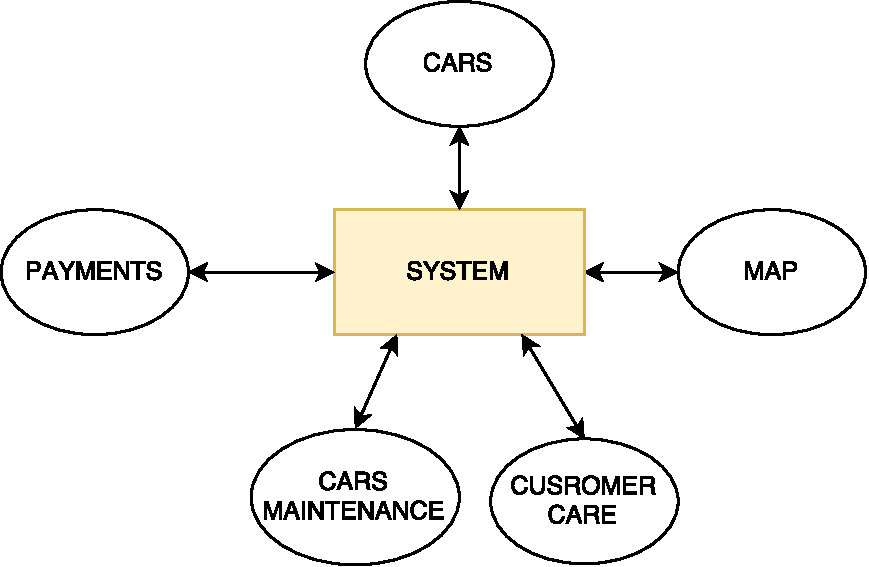
\includegraphics[scale=0.5]{system_blocks}
			\caption{
				\label{fig:systemInterfaces} 
				Overview of system interfaces
			}
		\end{figure}
	\paragraph{Payments}
	When a payment is required (e.g. when a user ends his rent) the system sends a request with all the details needed to complete the payment (i.d. name and surname of the user, due amount, credit card number etc.) to an external payment handling system. Once the external system completes the payment process, it sends our system the payment outcome so that the system can take appropriate action.
	
	\paragraph{Customer care} Every time it is required a customer care service operator can contact a user. Customer care service operators can request and see all user details, their rents and payments history. Such operators can also ban or unban users from the system, mark cars as not available and, in general, provide assistance to users.

	\paragraph{Maintenance} Every time a car requires maintenance, the system notifies an external pool of maintenance operators, providing  GPS position of the car and a brief description of the problem.

	\paragraph{Map} GPS position of cars and safe areas is displayed to all users, customer care operators and maintenance operators on a constantly updated map which relies on an external Geographic Information System.

	\paragraph{Cars}\label{sec:cars}All cars have modules that continuously provide communications between them and our system about:
	\begin{itemize}
		\item GPS position
		\item safe areas
		\item charging stations nearby current location
		\item engine status (on/off)
		\item number of passengers
		\item battery level (percentage)
		\item charging status (in charge/not in charge)
		\item door locking status (locked/unlocked)
		\item car status (see \autoref{fig:carFSA})
		\item current time
	\end{itemize}	
	The overall status of a car can be represented by an FSM
	\begin{figure}[h]
			\centering
			\includegraphics[scale=0.5]{CarFSA}
			\caption{
				\label{fig:carFSA} 
				Car statuses
			}
		\end{figure}
		
\subsubsection{User interfaces}
	Using the interfaces of the system users can:\todo{move car to system interface}
	\begin{enumerate}
		\item Register and log-in to the system
		\item On the map they can view the position of
			\begin{enumerate}[label=\alph*)]
				\item themselves
				\item safe areas
				\item available cars (with their current battery level)
				\item charging stations
			\end{enumerate}
		\item Reserve a car
		\item Ask the customer care service for assistance 
	\end{enumerate}
%	Using the interface in the car users can:
%	\begin{enumerate}
%		\item Start the engine
%		\item View the real time battery level
%		\item View their real time GPS position
%		\item View their position w.r.t safe areas
%		\item Terminate the rent\todo{through an interface? Must be so by definition!}
%		\item Ask the customer care service for assistance
%	\end{enumerate}			


	\todo{Move elsewhere}In order to use all feature of our system a user must be registered. All guest users can register to our system providing some relevant information about themselves (such as name, surname, phone number, driving license, payment details etc.). A registered user can reserve one\todo{Only one at a time! Check reqs} available car for 1 hour, in this period of time he can reach the car he reserved and once he is nearby...

\subsubsection{Software interfaces}
Databases and DBMSs are clearly required in order to store data about users, cars, charging stations, safe areas etc.

As mentioned before (see \autoref{sec:systemInterfaces}) the system needs to use external APIs and to expose interfaces in order to interact with other systems.

All vehicles have an embedded external software system, which is able to display all information described in \hyperref[sec:cars]{cars section}.

\subsection{Product functions}
	\todo{See goals?}The system will:
	\begin{enumerate}[label=\textbf{F\arabic*.}]
		\item Function 1
	\end{enumerate}

\subsection{User characteristics}
	Users can use our system when they want to rent a car.\\
	Necessary conditions for the user in order to use the system are:
	\begin{itemize}
		\item He must be able to use a smartphone
		\item He must be in the age of majority
		\item He must have a proper valid driving license
		\item He must be able to drive a car (i.d. he must be in both physical and mental health)
	\end{itemize}
	These conditions are approved by users during the registration to the system.

\subsection{Domain assumption}
	We assume that these assumptions hold true in the domain of our system 
	\begin{enumerate}[label=\textbf{DA\arabic*}]
		\item GPS position is supposed to be accurate
		\item GPS position and status of all cars is always available
		\item The user who reserves the car will always be the person who drives it
		\item Users are legally allowed to drive cars (i.d. users have a proper driving license)
		\item Charging stations are always working and continuously monitored by the system
		\item All data provided by users are correct and reliable
		\item All cars provided by the customer are equipped with a module which provides a set of
		primitives that allow the system to retrieve all the information it needs about the car and to 
		run commands which allow the system to  
	\end{enumerate}